\ifx\wholebook\relax \else

\documentclass[UTF8]{article}

\input{../common-zh-cn.tex}

\setcounter{page}{1}

\begin{document}

\title{递归}

\author{刘新宇
\thanks{{\bfseries 刘新宇} \newline
  Email: liuxinyu95@gmail.com \newline}
  }

\maketitle
\fi

\markboth{递归}{编程的数学原理}

\epigraph{\textbf{造物神}是\textbf{造}物主\textbf{物}色的\textbf{神}怪}{——[美]侯世达《哥德尔、埃舍尔、巴赫——集异壁之大成》}

\begin{wrapfigure}{R}{0.3\textwidth}
%\begin{figure}[htbp]
 \centering
 \includegraphics[scale=0.4]{img/Pythagoras.eps}
 \captionsetup{labelformat=empty}
 \caption{毕达哥拉斯(约前570——前490)}
 \label{fig:Pythagoras}
%\end{figure}
\end{wrapfigure}

人们通过深入了解数进而了解自然。在上一章中,我们介绍了自然数的皮亚诺公理。并且展示了一些和自然数有着相同结构的事物,包括计算机系统中的基本数据结构列表。自然数成为了我们进一步前进的基石。但是我们的大厦还不稳固。第一章中,我们不加证明地使用了递归的概念。例如阶乘的定义:

\[
\begin{array}{l}
fact(0) = 1 \\
fact(n + 1) = (n + 1) \cdot fact(n)
\end{array}
\]

以及$foldn$的实现:

\[
\begin{array}{l}
foldn(z, f, 0) = z \\
foldn(z, f, n') = f(foldn(z, f, n))
\end{array}
\label{eq:foldn}
\]

递归的原理是什么?为什么它是正确的?递归可以在更低的层次被表示么?这些都是我们在这一章要解决的问题。

\section{万物皆数}

从数出发研究世间万物的第一人要算是古希腊的数学家和哲学家毕达哥拉斯了。他的名字通过著名的勾股定理(在西方叫毕达哥拉斯定理)而家喻户晓。毕达哥拉斯出生于希腊的萨摩斯(Samos)岛,年轻时他曾去米利都(Miletus)向古希腊哲学的奠基人泰勒斯(Thales)学习。在泰勒斯的建议下,毕达哥拉斯前往东方学习数学。他在埃及学习了13年(一说为22年)。后来波斯帝国征服了埃及,他又随军向东到达了巴比伦,向巴比伦人学习数学和天文知识。或许后来他还到达了更远的印度。不论到了哪里,毕达哥拉斯都不断向有学问的人请教,丰富自己的见解。重要的是,他不仅刻苦学习,而且更善于思考。在经过兼收并蓄、汲取各家之长后,毕达哥拉斯形成并完善了自己的思想\cite{HanXueTao16}。

经历了漫长的在外游历后,这位年近半百的智者返回了故乡并开始讲学。公元前520年左右,为了摆脱当地的暴政,毕达哥拉斯移居到了意大利南部的克罗顿(Croton)发展,在那里他赢得了人们的信任与景仰。毕达哥拉斯的弟子中还有女性,他们把主要的精力都用来研究天文、几何、数论及音乐这四门学科。它们被称为四术(quadrivium),影响了欧洲教育两千多年\cite{StepanovRose15}。四术体现了毕达哥拉斯“万物皆数”的哲学思想。星体的运动与几何对应,而几何又以数为基础,数字还可以衍生出音乐。毕达哥拉斯是首个发现纯八度音(octave)在频率上有数学规律的人。他的弟子说他可以“听见天界的乐音”\footnote{关于毕达哥拉斯的逝世的说法不一。他领导的学派具有很高的声誉和政治影响,引起了敌对派的忌恨。后来受到民主运动的冲击,学派在克罗顿的活动场所遭到破坏。有人认为毕达哥拉斯被暴徒杀害,也有人说他逃到梅塔蓬图姆(Metapontum)并度过余生。}。

毕达哥拉斯学派深入研究了数与数、数与自然之间的关系。这开启了数学的重要分支——数论。他们对正整数进行了分类,定义了奇数偶数、素数和数等。他们发现某些数的所有真因子\footnote{小于数本身的因子}之和恰好等于这个数本身,毕达哥拉斯学派称这样的数为完全数,并成功地找到两个\footnote{一说为完美数。经过欧几里得与欧拉的进一步工作,揭示了偶完全数的特征以及完全数和梅森素数的关系。到2018年,人们借助计算机共发现了50个梅森素数和完全数。}。最小的完全数是6,因为6 = 1 + 2 + 3,下一个是28(等于1 + 2 + 4 + 7 + 14)。毕达哥拉斯学派还发现了一大类“形数”(figurate number)\footnote{毕达哥拉斯学派的门徒通过在地上摆小石子来研究数字,英文的计算calculus一词就是从希腊文“石子”衍生出的\cite{HanXueTao16}。当他们把石子按照某种几何方式排列成图形时,就得到了形数。}。

\begin{figure}[htbp]
%\begin{wrapfigure}{R}{0.4\textwidth}
\centering
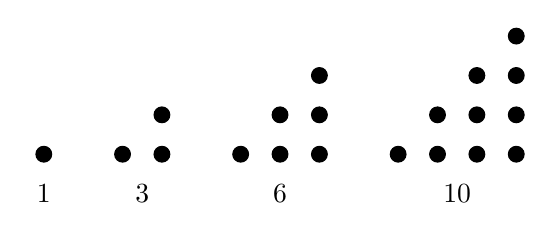
\begin{tikzpicture}[scale=0.5]
\filldraw (0, 0) circle (0.2);
\draw (0, -1) node{1};
\filldraw (2, 0) circle (0.2)
          (3, 0) circle (0.2)   (3, 1) circle (0.2);
\draw (2.5, -1) node{3};
\filldraw (5, 0) circle (0.2)
          (6, 0) circle (0.2)   (6, 1) circle (0.2)
          (7, 0) circle (0.2)   (7, 1) circle (0.2)   (7, 2) circle (0.2);
\draw (6, -1) node{6};
\filldraw (9, 0) circle (0.2)
          (10, 0) circle (0.2)    (10, 1) circle (0.2)
          (11, 0) circle (0.2)    (11, 1) circle (0.2)    (11, 2) circle (0.2)
          (12, 0) circle (0.2)    (12, 1) circle (0.2)    (12, 2) circle (0.2)    (12, 3) circle (0.2);
\draw (10.5, -1) node{10};
\end{tikzpicture}
\caption{三角形数(triangular number)}
\label{fig:triangular-num}
%\end{wrapfigure}
\end{figure}

\begin{figure}[htbp]
%\begin{wrapfigure}{R}{0.4\textwidth}
\centering
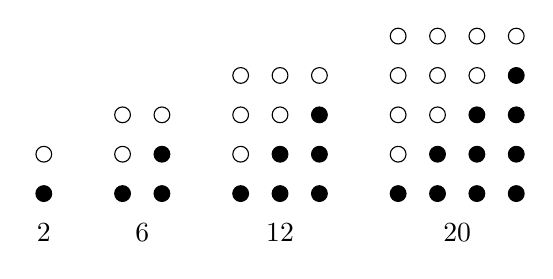
\begin{tikzpicture}[scale=0.5]
\draw (0, 1) circle (0.2);
\filldraw (0, 0) circle (0.2);
\draw (0, -1) node{2};

\draw (2, 1) circle (0.2)   (2, 2) circle (0.2)
      (3, 2) circle (0.2);
\filldraw (2, 0) circle (0.2)
          (3, 0) circle (0.2)   (3, 1) circle (0.2);
\draw (2.5, -1) node{6};

\draw (5, 1) circle (0.2)   (5, 2) circle (0.2)   (5, 3) circle (0.2)
      (6, 2) circle (0.2)   (6, 3) circle (0.2)
      (7, 3) circle (0.2);
\filldraw (5, 0) circle (0.2)
          (6, 0) circle (0.2)   (6, 1) circle (0.2)
          (7, 0) circle (0.2)   (7, 1) circle (0.2)   (7, 2) circle (0.2);
\draw (6, -1) node{12};

\draw (9, 1) circle (0.2)   (9, 2) circle (0.2)   (9, 3) circle (0.2)   (9, 4) circle (0.2)
      (10, 2) circle (0.2)   (10, 3) circle (0.2)   (10, 4) circle (0.2)
      (11, 3) circle (0.2)   (11, 4) circle (0.2)
      (12, 4) circle (0.2);
\filldraw (9, 0) circle (0.2)
          (10, 0) circle (0.2)    (10, 1) circle (0.2)
          (11, 0) circle (0.2)    (11, 1) circle (0.2)    (11, 2) circle (0.2)
          (12, 0) circle (0.2)    (12, 1) circle (0.2)    (12, 2) circle (0.2)    (12, 3) circle (0.2);
\draw (10.5, -1) node{20};
\end{tikzpicture}
\caption{长方形数(oblong number)}
\label{fig:oblong-num}
%\end{wrapfigure}
\end{figure}

图\ref{fig:triangular-num}和图\ref{fig:oblong-num}分别是三角形数和长方形数。很容易看出,每个长方形数都是对应三角形数的二倍,而三角形数又是前$n$个正数之和,因此就得到了正整数累加的求和公式:

\[
1 + 2 + 3 + ... + n = \frac{1}{2}n(n+1)
\]

毕达哥拉斯学派还观察到,所有的奇数可以标示成折尺形(数学上称为“磬折形”),如图\ref{fig:gnomon-num},而前$n$个折尺形可以拼成一个正方形,如图\ref{fig:square-num}。这样他们就发现了前$n$个正奇数的求和公式:

\[
1 + 3 + 5 + ... + (2n - 1) = n^2
\]

\begin{figure}[htbp]
%\begin{wrapfigure}{R}{0.4\textwidth}
\centering
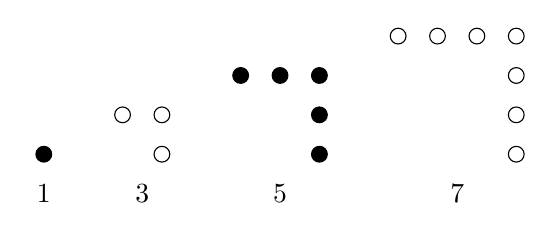
\begin{tikzpicture}[scale=0.5]
\filldraw (0, 0) circle (0.2);
\draw (0, -1) node{1};

\draw (2, 1) circle (0.2)
      (3, 0) circle (0.2)   (3, 1) circle (0.2);
\draw (2.5, -1) node{3};

\filldraw (5, 2) circle (0.2)   (6, 2) circle (0.2)   (7, 2) circle (0.2)
          (7, 0) circle (0.2)   (7, 1) circle (0.2);
\draw (6, -1) node{5};

\draw (9, 3) circle (0.2)   (10, 3) circle (0.2)   (11, 3) circle (0.2)   (12, 3) circle (0.2)
      (12, 0) circle (0.2)    (12, 1) circle (0.2)    (12, 2) circle (0.2);
\draw (10.5, -1) node{7};
\end{tikzpicture}
\caption{折尺形数(gnomon number)}
\label{fig:gnomon-num}
%\end{wrapfigure}
\end{figure}

\begin{figure}[htbp]
%\begin{wrapfigure}{R}{0.4\textwidth}
\centering
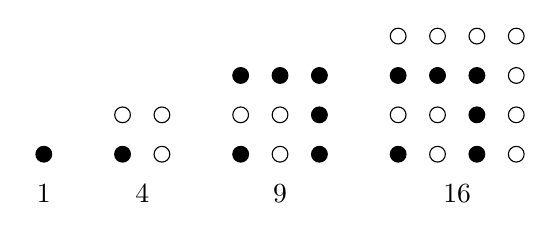
\begin{tikzpicture}[scale=0.5]
\filldraw (0, 0) circle (0.2);
\draw (0, -1) node{1};

\filldraw (2, 0) circle (0.2);
\draw (2, 1) circle (0.2)
      (3, 0) circle (0.2)   (3, 1) circle (0.2);
\draw (2.5, -1) node{4};

\filldraw (5, 0) circle (0.2);
\draw (5, 1) circle (0.2)
      (6, 0) circle (0.2)   (6, 1) circle (0.2);
\filldraw (5, 2) circle (0.2)   (6, 2) circle (0.2)   (7, 2) circle (0.2)
          (7, 0) circle (0.2)   (7, 1) circle (0.2);
\draw (6, -1) node{9};

\filldraw (9, 0) circle (0.2);
\draw (9, 1) circle (0.2)
      (10, 0) circle (0.2)   (10, 1) circle (0.2);
\filldraw (9, 2) circle (0.2)   (10, 2) circle (0.2)   (11, 2) circle (0.2)
          (11, 0) circle (0.2)   (11, 1) circle (0.2);
\draw (9, 3) circle (0.2)   (10, 3) circle (0.2)   (11, 3) circle (0.2)   (12, 3) circle (0.2)
      (12, 0) circle (0.2)    (12, 1) circle (0.2)    (12, 2) circle (0.2);
\draw (10.5, -1) node{16};
\end{tikzpicture}
\caption{正方形数(square number)与折尺形数的关系}
\label{fig:square-num}
%\end{wrapfigure}
\end{figure}

这正是我们在第一章提出的那个练习题的答案。就这样,毕达哥拉斯学派发现,很多事物和现象都可以从数的方面进行说明和解释。例如,具有同样张力的两根弦,当它们的长度为简单的整数比时,奏出的乐声就和谐悦耳。由此毕达哥拉斯发展出了最初的音乐理论。音乐与数这似乎毫无关联的两者间存在的这种意外联系,给毕达哥拉斯很大影响。他从中得到启发并大胆推测:所有的事物都可以用整数或整数的比来解释。毕达哥拉斯学派开始热衷与用数去解释更多的现象,他们相信宇宙的本质就在于“数的和谐”,并且提出“万物皆数”的论断。由此出发,毕达哥拉斯学派试图发展一套以数字为基础的理论,使得几何学可以建立在该理论之上。这种想法实际上就相当于要创建一套基于正整数的统一数学理论。

毕达哥拉斯学派最著名的发现当属勾股定理的证明。至今这一定理在西方仍被称为“毕达哥拉斯定理”。然而,我们将看到勾股定理是一把双刃剑,他的结果最终形成了一个递归的怪圈,使得“万物皆数”的理念出现了漏洞。为此,我们先要引出可公度概念和欧几里得算法。为了将几何纳入“万物皆数”的理论,毕达哥拉斯学派提出了一个概念来定义一条线段可以用另一条线段来度量。这个定义说,如果一条线段A可以通过有限的连续的另一条线段V来表示时,线段V可用于线段A的量度(measure)。这本质上是说,我们可以通过整数次拼接产生另一条线段。尽管度量两条不同的线段时,可以使用各自的量度,但是如果想用同一量度测量不同的线段,它必须是二者的公度(common measure)。即当且仅当线段V可以同时成为线段A和线段B的量度时,它才能成为二者的公度。毕达哥拉斯学派认为,任何情况下都可以找到公度,这样几何就可以建立在整数之上了。

%\begin{wrapfigure}{R}{0.4\textwidth}
\begin{figure}[htbp]
 \centering
 \includegraphics[scale=0.2]{img/Pythagoras-proof.eps}
 \caption{勾股定理的一种几何证明,两幅图中白色面积相等(来自《周髀算经》,约公元前200年)}
 \label{fig:Pythagoras-proof}
\end{figure}
%\end{wrapfigure}

\section{欧几里得算法}

公度的概念,无理数的发现和递归的关系。

%\begin{wrapfigure}{R}{0.4\textwidth}
%% \begin{figure}[htbp]
%%  \centering
%%  \includegraphics[scale=0.2]{img/Peano.eps}
%%  \caption{朱塞佩$\cdot$皮亚诺(Giuseppe Peano)1858 - 1932。}
%%  \label{fig:Peano}
%% \end{figure}
%\end{wrapfigure}

欧几里得最大公约数(公度)算法的概念。几何量和数的分离。最大公约数算法的意义,递归原理问题的提出

扩展欧几里得算法、倒水趣题。

\section{$\lambda$演算}

lambda的由来,三大变换:Alpha, Beta, Eta变换,变换与归约。

%\begin{figure}[htbp]
\begin{wrapfigure}{R}{0.4\textwidth}
\centering
\begin{tikzpicture}[scale=0.8]
\filldraw[fill=gray, draw=black, pattern=north west lines] (0, 0) rectangle (2, 1)
    (2, 0) rectangle (3, 1);
\draw (3, 0) rectangle (4.5, 1);
\draw (0, -1) rectangle (2, -2);
\filldraw[fill=gray, draw=black, pattern=north west lines] (2, -1) rectangle (3, -2)
    (3, -1) rectangle (4.5, -2);
\end{tikzpicture}
\caption{加法结合律的几何证明。上下面积相等}
\end{wrapfigure}
%\end{figure}

%\begin{wrapfigure}{R}{0.4\textwidth}
\begin{figure}[htbp]
\centering
\begin{tikzpicture}[scale=0.8]
\draw (0, 0) rectangle (2, 1)
    (2, 0) rectangle (3, 1);
\draw (0, -1) rectangle (1, -2)
    (1, -1) rectangle (3, -2);
\end{tikzpicture}
\caption{加法交换律的几何证明。将上方的图形倒过来看,或者在镜中看。}
\end{figure}
%\end{wrapfigure}

\begin{Exercise}
\begin{enumerate}
\item 一些lambda演算的练习
\end{enumerate}
\end{Exercise}

\section{递归的定义}

Y组合子和递归的定义
%% \begin{wrapfigure}{R}{0.4\textwidth}
%% %\begin{figure}[htbp]
%%  \centering
%%  \includegraphics[scale=0.4]{img/Fibonacci.eps}
%%  \caption{比萨的列奥纳多,又称斐波那契(Leonardo Pisano, Fibonacci),1175年-1250年}
%%  \label{fig:Fibonacci}
%% %\end{figure}
%% \end{wrapfigure}


%\begin{wrapfigure}{L}{0.3\textwidth}
%% \begin{figure}[htbp]
%%  \centering
%%  \includegraphics[scale=0.5]{img/fibonacci_spiral.eps}
%%  \caption{这些正方形的边长组成了斐波那契序列。}
%%  \label{fig:fibonacci_spiral}
%% \end{figure}
%\end{wrapfigure}

%\begin{wrapfigure}{R}{0.3\textwidth}
%% \begin{figure}[htbp]
%%  \centering
%%  \includegraphics[scale=0.2]{img/PWW.eps}
%%  \caption{《无需语言的证明》封面局部}
%%  \label{fig:PWW}
%% \end{figure}
%\end{wrapfigure}

\section{$\lambda$的意义}

CONS/HEAD/TAIL的lambda表示。

二叉树、多叉树的递归结构与FOLD

\section{递归的结构与形式}

%\begin{wrapfigure}{R}{0.3\textwidth}
%% \begin{figure}[htbp]
%%  \centering
%%  \includegraphics[scale=1.0]{img/the-school-of-athens.eps}
%%  \caption{拉斐尔《雅典学院》局部}
%%  \label{fig:the-school-of-athens}
%% \end{figure}
%\end{wrapfigure}

递归的形式之美——分形与艺术

递归的结构之美——文艺和音乐作品

\ifx\wholebook\relax \else
\begin{thebibliography}{99}

\bibitem{HanXueTao16}
韩雪涛 ``数学悖论与三次数学危机''. 人民邮电出版社. 2016, ISBN: 9787115430434

\bibitem{StepanovRose15}
[美] 亚历山大 A$cdot$斯捷潘诺夫,丹尼尔 E$\cdot$罗斯著,爱飞翔译. ``数学与泛型编程:高效编程的奥秘''. 机械工业出版社. 2017, ISBN: 9787111576587

\end{thebibliography}

\expandafter\enddocument
%\end{document}

\fi
